\documentclass[12pt]{article}
\linespread{1.25}
\usepackage{times}

\usepackage{pgfplots}
\pgfplotsset{compat = newest}
\usetikzlibrary{positioning, arrows.meta}
\usepgfplotslibrary{fillbetween}
\usepackage{amsmath}

\begin{document}

\begin{center}
\hspace*{-3cm}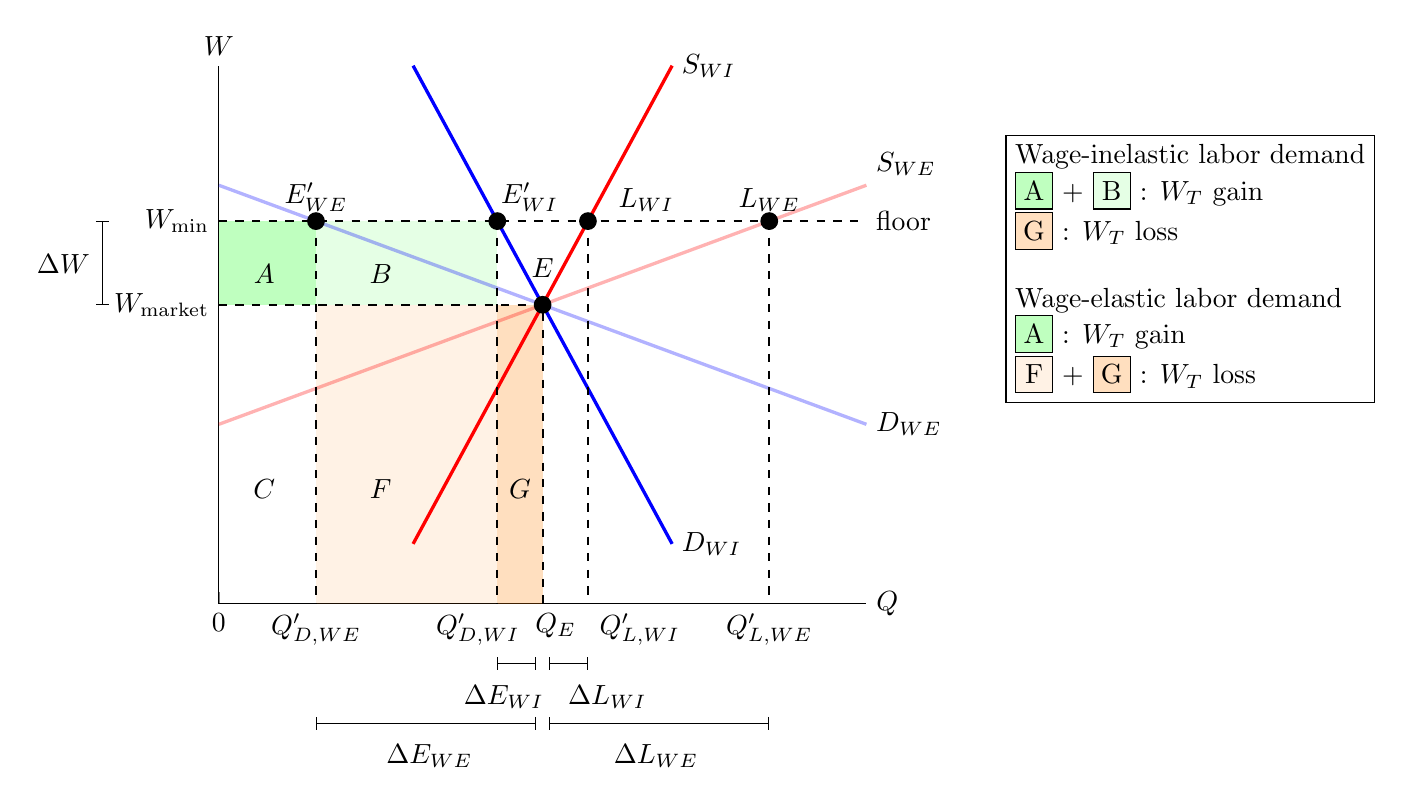
\begin{tikzpicture}
\begin{axis}[
scale = 1.2,
xmin = 0, xmax = 10,
ymin = 2.5, ymax = 7,
axis lines* = left,
xtick = {0}, ytick = \empty,
clip = false,
]
% Colouring areas
\fill[green, opacity = 0.25] (0, 5.7) -- (1.5, 5.7) -- (1.5, 5) -- (0, 5);
\fill[green, opacity = 0.1] (1.5, 5.7) -- (1.5, 5) -- (4.3, 5) -- (4.3, 5.7);
\fill[orange, opacity = 0.25] (4.3, 2.5) -- (5, 2.5) -- (5, 5) -- (4.3, 5);
\fill[orange, opacity = 0.1] (4.3, 2.5) -- (4.3, 5) -- (1.5, 5) -- (1.5, 2.5);

% Supply and Demand Curves
\node [above] at (current axis.above origin) {$W$};
\node [right] at (current axis.right of origin) {$Q$};
\addplot[color=blue, very thick, opacity=0.3] coordinates {(0,6)(10,4)};
\addplot[color=blue, very thick] coordinates {(3,7)(7,3)};
\addplot[color=red, very thick, opacity=0.3] coordinates{(0,4)(10,6)};
\addplot[color=red, very thick] coordinates{(3,3)(7,7)};

% Wage Floor
\addplot[color=black, dashed, thick] coordinates {(0,5.7)(10,5.7)};

% Quantity and Price Lines
\addplot[color=black, dashed, thick] coordinates {(0,5)(5,5)(5,2.5)};
\addplot[color=black, dashed, thick] coordinates {(1.5,5.7)(1.5,2.5)};
\addplot[color=black, dashed, thick] coordinates {(4.3,5.7)(4.3,2.5)};
\addplot[color=black, dashed, thick] coordinates {(5.7,5.7)(5.7,2.5)};
\addplot[color=black, dashed, thick] coordinates {(8.5,5.7)(8.5,2.5)};

% Labels: E, L
\addplot[color=black, mark=*, only marks, mark size=3pt] coordinates {(1.5, 5.7)(4.3,5.7)(5,5)(5.7, 5.7)(8.5,5.7)};
\node [above=2pt] at (5, 5.1) {$E$};
\node [above] at (1.5, 5.7) {$E^{\prime}_{WE}$};
\node [above] at (4.8, 5.7) {$E^{\prime}_{WI}$};
\node [above] at (6.6, 5.7) {$L_{WI}$};
\node [above] at (8.5,5.7) {$L_{WE}$};

% Labels: S, D
\node [right] at (10, 4) {$D_{WE}$};
\node [above right] at (10, 6) {$S_{WE}$};
\node [right] at (7, 3) {$D_{WI}$};
\node [right] at (7, 7) {$S_{WI}$};
\node [left] at (0, 5) {$W_{\text{market}}$};
\node [left] at (0, 5.7) {$W_{\text{min}}$};
\node [below] at (1.5, 2.5) {$Q^{\prime}_{D, WE}$};
\node [below] at (4, 2.5) {$Q^{\prime}_{D, WI}$};
\node [below] at (5.2, 2.5) {$Q_E$};
\node [below] at (6.5, 2.5) {$Q^{\prime}_{L, WI}$};
\node [below] at (8.5, 2.5) {$Q^{\prime}_{L, WE}$};
\node [right] at (10, 5.7) {floor};
\node [above] at (0.7, 5.1) {$A$};
\node [above] at (0.7, 3.3) {$C$};
\node [above] at (2.5, 5.1) {$B$};
\node [above] at (2.5, 3.3) {$F$};
\node [above] at (4.65, 3.3) {$G$};

% Dimension indicators
\draw[|-|] (4.3, 2) -- (4.9, 2);
\node [below] at (4.4, 1.9) {$\Delta E_{WI}$};
\draw[|-|] (5.1, 2) -- (5.7, 2);
\node [below] at (6, 1.9) {$\Delta L_{WI}$};
\draw[|-|] (1.5, 1.5) -- (4.9, 1.5);
\node [below] at (3.25, 1.4) {$\Delta E_{WE}$};
\draw[|-|] (5.1, 1.5) -- (8.5, 1.5);
\node [below] at (6.75, 1.4) {$\Delta L_{WE}$};
\draw[|-|] (-1.8, 5) -- (-1.8, 5.7);
\node [below] at (-2.4, 5.5) {$\Delta W$};

% Legend
\node[draw, align=left] at (15, 5.3){
Wage-inelastic labor demand \\
\fcolorbox{black}{green!25}{\makebox[\fontcharht\font`X]{A}} + \fcolorbox{black}{green!10}{\makebox[\fontcharht\font`X]{B}} : $W_T$ gain \\
\fcolorbox{black}{orange!25}{\makebox[\fontcharht\font`X]{G}} : $W_T$ loss \\ \\
Wage-elastic labor demand \\
\fcolorbox{black}{green!25}{\makebox[\fontcharht\font`X]{A}} : $W_T$ gain \\
\fcolorbox{black}{orange!10}{\makebox[\fontcharht\font`X]{F}} + \fcolorbox{black}{orange!25}{\makebox[\fontcharht\font`X]{G}} : $W_T$ loss 
};
\end{axis}
\end{tikzpicture}\hspace*{-3cm}
\end{center}
\textbf{Figure 0-1:} Wage elasticities and total income.

\end{document}